% background
% brief review of previous research (cite)
% reson why the research was undertaken
% Hypothesis
% explenation of techniques and why they ve been chosen
% objectives = what you hope to achieve
% brief reference to the main outcome

%$\ce{CdS_x Se_{1-x}/ZnS}$



\section{Introduction}
\label{sec:Introduction}

As the resistivity of metals and semiconductors depends on the temperature in different ways,
here a temperature dependent resistance measurement is done in order to characterize the samples of 
(R1)N-doped germanium, (R2)copper and (R3)nickel, where the germanium represents a semiconductor.

The resistance $R$ can be measured as a voltage drop $V$ over a sample with current $I$.
The aim of a resistivity ($\rho$) measurement is to derive the resistivity of the material, which is defined as the reciprocal of the conductivity

\begin{equation}\label{eq:rho}
    \sigma = 1 / \rho = J / E = q n \mu,
\end{equation}
where $J$ is the current density and $E$ the electric field intensity.
Further, $q$ is the elemtary charge, $\mu$ the charge carrier mobility and $n$ the carrier density.
Here, the macroscopic definition is based on a microscopic model for carrier mobility.
Another definition of the resistivity for uniform samples is given by 
\begin{equation}
    \rho = R S / L,
\end{equation}
where L is the length of the sample and S its cross-section.

As the material characteristic parameters $n$ and $\mu$ behave different according to temperature changes in metals and semiconductors, some conciderations have to be done.
The mobility decreases with temperature 
\begin{equation}\label{eq:metal}
  \mu \propto T^{-1}.
\end{equation}
For metals, the carrier density is constant whereas for doped semiconductors this is only true for the extrinsic region carriers.
Instead, the intrinsic reagion carrier density can be described as a exponential correlation
\begin{equation}\label{eq:intrinsic}
  n_i \propto \exp{-E_g /2k_bT},
\end{equation}
where $E_g$ is the semiconductors energy gap and $k_b$ the Boltzmann constant.
Summing up, the expected relation for metals is $\rho \propto T$ (\ref{eq:rho}, \ref{eq:metal}), for semiconductors in a low temperature domain
a metal-like behavior and for high temperatures an exponential decreasing of the resistivity is expected \ref{eq:rho}, \ref{eq:intrinsic}.

\subsection{Experimental setup}
\label{sec:setup}

\begin{figure*}
  \centering
  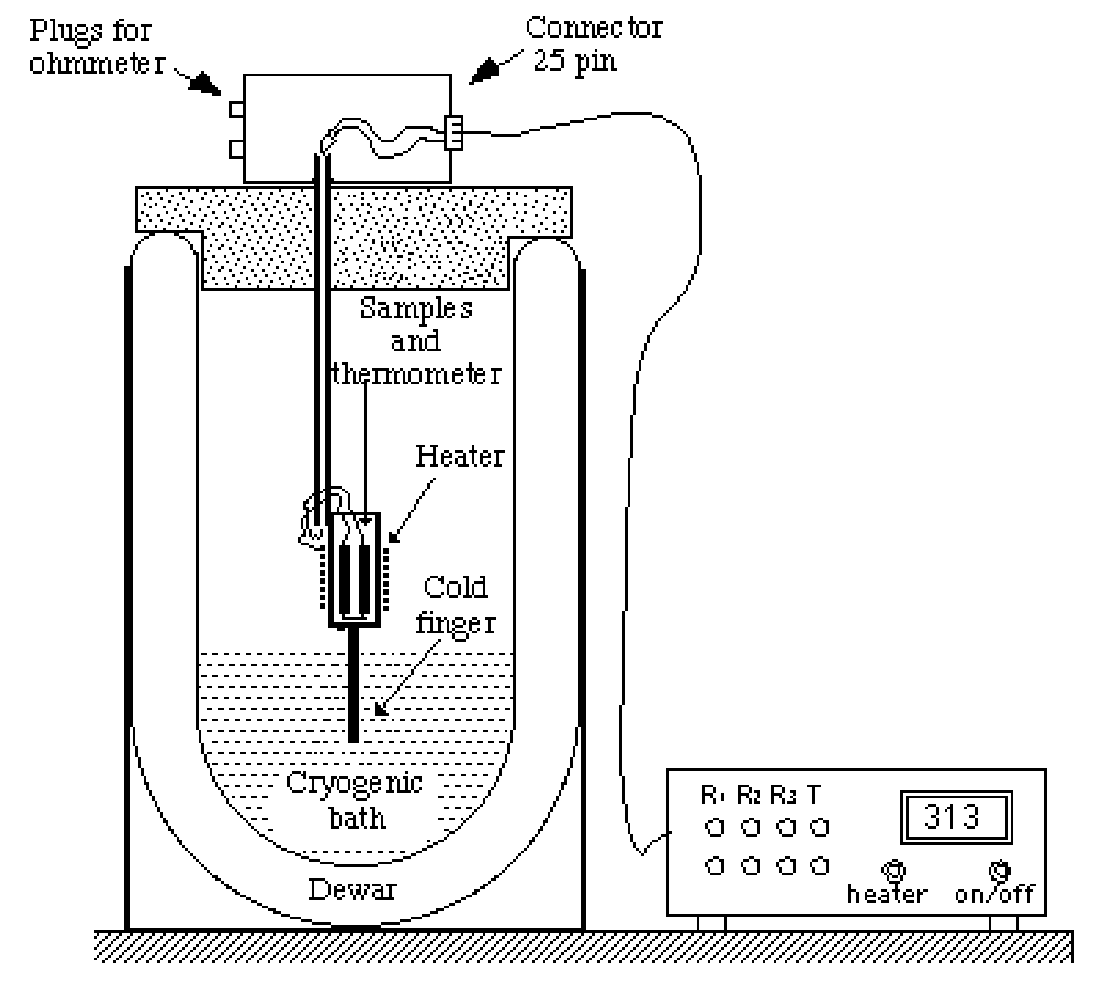
\includegraphics[width=0.55\textwidth]{graphics/setup.png}
  \caption[width=0.4\textwidth]{Schematic setup of the experiment\cite{instruction}.}
  \label{fig:setup}
\end{figure*}

The apperatus includes three samples, and allows time resolved, temperature dependend resistance measurements.
As depicted schematically in figure \ref{fig:setup}, the samples are inside a brass sampleholder which can be cooled down by bringing the cold finger in contact with liquid nitrogen.
Therefore, the whole apperatus is positioned into a dewar.
A $\SI{50}{\ohm}$ heater is installed inside the sampleholder to reach temperatures up to $\SI{450}{\kelvin}$.

The samples are wired inside the sampleholder and connected to a controlunit.
Also a thermometer is installed to overlook the current sample temperature.

The controlunit is providing power supply to the heater, the samples current bias and to the therometer.

In technical detail, the absolute temperature T is measured by the forward voltage of a PN junction on constant current bias. 
The samples resistance measurement is done by using a four wires volt-amperometric architecture mentioned in chapter \ref{sec:R-measurement}. 
Here, in order to eliminate the effect of wire and contact resistance, the current supply is separated by the voltage measurement by using four wires instead of two.

The metallic samples are thin wires with a nominal diameter of $\SI{0.05}{\milli\meter}$ and a few centimeters long, whereas the germanium sample is a $\SI{1}{\milli\meter}$ thick wafer, cut into a $\SI{3}{\milli\meter} \times \SI{5}{\milli\meter}$ plate.
The bias currents are $\SI{1}{\milli\ampere}$ for germanium, $\SI{2}{\milli\ampere}$ for nickel and $\SI{10}{\milli\ampere}$ for copper.

To amplify the differential voltage signal along the sample a high input impedance operational amplifier (INA114) with sample dependant gain G is used.
The choosen values are $G_1 = 100, G_2=10$ and $G_3=1$, which is reciprocal to the sensitivity of the output voltage measurement.
The temperature channel has a sensitivity of $\SI{10}{\milli\volt\per\kelvin}$ in the temperature range of the experiment.

To use the LoggerPro aquisition program on the PC, the LabPro surface is used. 
The aquisition module is connected by a standard 25-pin cable to the PC.

The samples are also connected to four banana plugs, where they are called S1,S2,S3 and GND.
Therefore, it is possible to measure the resistance by the two wires technique mentioned in chapter \ref{sec:R-measurement}.
Also a four wires resistance measurement, as elaborated in chapter \ref{sec:R-measurement} can be done.

\subsection{Resistivity measurement circuits}
\label{sec:R-measurement}

\begin{figure*}
  \centering
  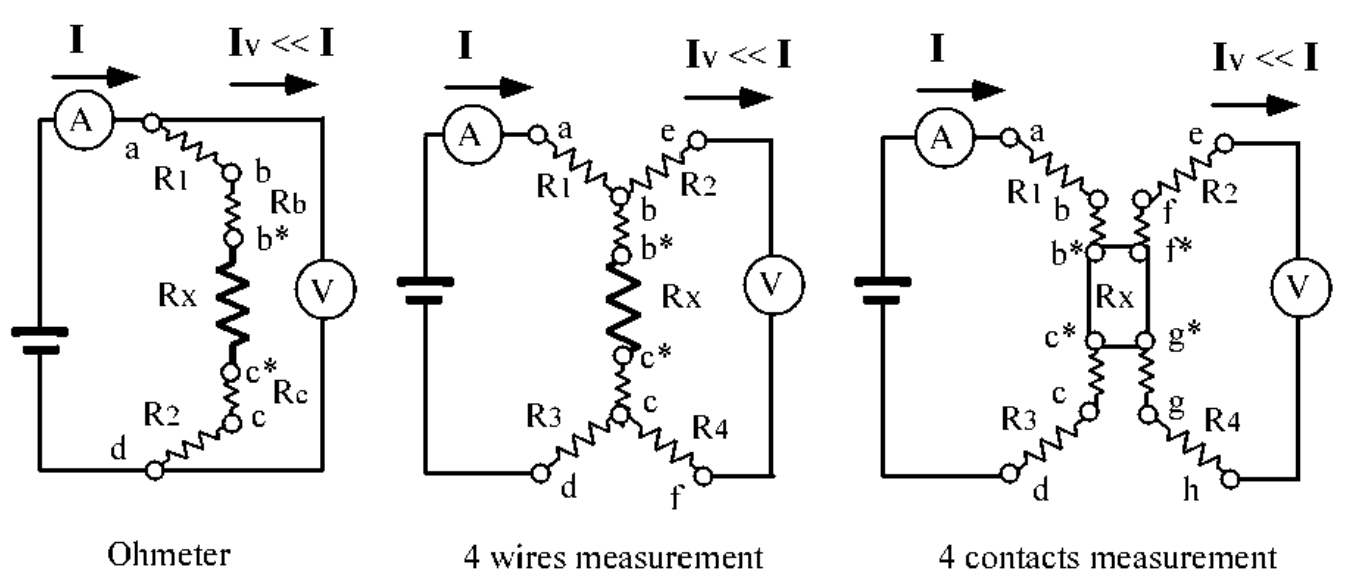
\includegraphics[width=0.7\textwidth]{graphics/r-measure.png}
  \caption[width=0.7\textwidth]{Different techniques for measuring the resistance Rx \cite{instruction}.}
  \label{fig:resistance-measure}
\end{figure*}

As one can find depicted in figure \ref{fig:resistance-measure} there are several circuits allowing resistance measurements in an either technical easy or precise way.
The easiest is the ohmmeter - two wire circuit. 
Measuring the voltage drop for a set current, results in a resistance measurement not only for the sample, but adds in series the contact- and wireresistance.
  
This systematic error of wire resistance can be outrun by using the 4 wires measurement architecture.
Here, the current $I_V$ produces a neglectable voltage drop along $R_1$ and $R_2$.
The high voltage across $R_1$ and $R_3$, which are current feeding do not affect the measurement.
Still, the contact resistance is in series with the to be measured Rx and thus, can not be neglected.

The 4 contacts measurement uses the sample principle as the 4 wires measurement to outrun also the contact resistance, as seen in figure \ref{fig:resistance-measure}.
Especially, for a semiconductor where the contact resistance is high, this technique may be the one of choice.

\subsection{Resistivity of wires}
\label{sec:wires-theo}

This part of the experiment can be seen seperately, but allows to proof the functionality of the two- and four-wire resistance measurement mentioned in chapter \ref{sec:R-measurement}.
Therefore, four wires made from unknown material are analyzed in terms of resitance.
This is done for all samples for both measurement setups for five lenghts of the wire.
For this measurement a Sourcemeter 2400 is used.

For both methods the material specific resistity can be caluclated as 
\begin{equation}
  \rho = R \frac{\pi r^2}{L},
\end{equation}\label{equ:wires}
where $r$ is the radius of the wire and L the length.
By knowing the resistivity, which is a material specific quantity, an estimation of the wire`s material can be done.
